\documentclass{llncs}
\usepackage{makeidx}
\usepackage{enumerate}
\usepackage[dvips,dvipdfm]{epsfig}
\usepackage{authblk}
\usepackage{subfigure}
\usepackage{amssymb}
\usepackage{amsmath}
\usepackage{amsfonts}
\usepackage{booktabs}
\usepackage{threeparttable}
\usepackage{algorithm}
\usepackage{algorithmicx}
\usepackage{algpseudocode}
\usepackage{textcomp}
\usepackage{fancyhdr}
\pagestyle{fancy}
\fancyhf{}
\renewcommand{\headrulewidth}{0pt}
\renewcommand{\footrulewidth}{0pt}
\renewcommand{\algorithmicrequire}{\textbf{Input}}
\renewcommand{\algorithmicensure}{\textbf{Output}}
\fancyhead[RO]{{\scriptsize RORM: The Matrix of Refined Ordering Relations with Uncertainty \qquad\thepage}}
\fancyhead[LE]{{\scriptsize \thepage\qquad Shuhao Wang, Lijie Wen, Zixuan Wang, Jianmin Wang and Jianwen Su}}
\begin{document}
\frontmatter 
\addtocmark{RORM}

\mainmatter
\title{RORM: a Behavioral Process Model Similarity Measure based on the Matrix of Refined Ordering Relations with Uncertainty}
\titlerunning{RORM: a Behavioral Process Model Similarity Measure based on the Matrix of Refined Ordering Relations with Uncertainty}

\author[$\$$]{Shuhao Wang}
\author[$\$$]{Lijie Wen}
\author[$\$$]{Zixuan Wang}
\author[$\$$]{Jianmin Wang}
\author[$\#$]{Jianwen Su}
\authorrunning{Shuhao Wang et al.}
\tocauthor{Shuhao Wang, Lijie Wen, Zixuan Wang, Jianmin Wang and Jianwen Su}
\affil[$\$$]{School of Software, Tsinghua University, Beijing 100084, P.R. China \authorcr
\texttt{shudiwsh2009@gmail.com,wenlj@tsinghua.edu.cn,
iamwangzixuan@hotmail.com,jimwang@tsinghua.edu.cn}}
\affil[$\#$]{Department of Computer Science, UC Santa Barbara, USA \authorcr
\texttt{su@cs.ucsb.edu}}
\institute{}

\maketitle

\begin{abstract}
With continuous development of the Business Process Management (i.e. BPM) and the innovation of the workflow technology, the scale of large organizations and enterprises process model repositories is increasing. Their effective utilization requires an effective retrieval mechanism, so the analysis of the similarity between models is proposed as indispensable. Existing measures for process model similarity have various limitations. In this paper, we introduce a new metric to quantify process similarity based on the refined ordering relations with uncertainty. It uses Jaccard coefficient to measure the similarity between the sets of behavioral relation pairs of process model activities. Experiments show that our measure is both efficient and effective.
\keywords{Business Process Model, Refined Ordering Relations with Uncertainty, Sequential Direct Adjacency, Behavioral Similarity}
\end{abstract}

\section{Introduction}\label{sec:introduction}

\section{Preliminaries}\label{sec:preliminaries}
Our work is to measure the similarity between two process models. We will show our algorithm on a specific type of process model named Petri net.

The concept of the Petri net has its origin in Carl Adam Petri's dissertation \cite{petri1966kommunikation}. Petri nets are a graphical and mathematical modeling tool applicable to many systems. They are a promising tool for describing and studying information processing systems that are characterized as being concurrent, asynchronous, distributed, parallel, nondeterministic, and/or stochastic \cite{murata1989petri}.

\begin{definition}[Petri net]\label{def:petrinet}
A Petri net is a 5-tuple, $PN=(P,T,F,W,M_{0})$ where:
	\begin{itemize}
		\item[] $P=\{p_{1},p_{2},...,p_{m}\}$ is a finite set of places,
		\item[] $T=\{t_{1},t_{2},...,t_{n}\}$ is a finite set of transitions,
		\item[] $F\subseteq(P\times T)\cup(T\times P)$ is a set of arcs (flow relation),
		\item[] $W:F\rightarrow\{1,2,3,...\}$ is a weight function,
		\item[] $M_{0}:P\rightarrow\{0,1,2,3,...\}$ is the initial marking,
		\item[] $P\cap T=\emptyset$ and $P\cup T\neq\emptyset$.
	\end{itemize}
A Petri net structure $N=(P,T,F,W)$ without any specific initial marking is denoted by $N$. A Petri net with the given initial marking is denoted by $(N,M_{0})$.
\end{definition}

\begin{figure}[H]
	\centering
	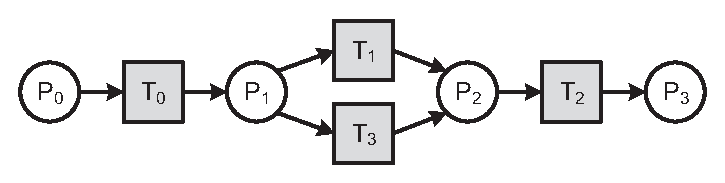
\epsfig{file=petri_example.eps,width=0.7\textwidth}
	\caption{A example of Petri net\label{fig:exPetri}}
\end{figure}

Figure \ref{fig:exPetri} shows an example of Petri net. For more details, please refer to the work of Murata \cite{murata1989petri}. A Petri net which models a workflow process definition is called a WorkFlow net (WF-net) \cite{van1998application}.

\begin{definition}[WF-net]\label{def:wfnet}
A Petri net $PN=(P,T,F)$ is a WF-net (Workflow net) if and only if:
	\begin{enumerate}[(i)]
		\item $PN$ has two special places: $i$ and $o$. Place $i$ is a source place: $\bullet i=\emptyset$. Place $o$ is a sink place: $o\bullet =\emptyset$.
		\item If we add a transition $t^{*}$ to $PN$ which connects place $o$ with $i$ (i.e. $\bullet t^{*}=\{o\}$ and $t^{*}\bullet=\{i\}$), then the resulting Petri net is strongly connected.
	\end{enumerate}
\end{definition}

We extract the relations between activities on WF-net. A intuitive idea is to generate all the full firing sequences (or traces) of a model, which will be infinite in a model with loop structures. Also, we need to consider all possible interleavings of concurrent events, which causes the state explosion problem in a concurrent system \cite{mcmillan1995technique}. Javier Esparza proposed the notion of complete finite prefix to avoid this \cite{esparza1996improvement}, based on the improvement of MaMillan's unfolding algorithm \cite{mcmillan1995technique}.



% \section{Refined Ordering Relations with Uncertainty}\label{sec:relations}

% \section{Similarity Measure}\label{sec:similarity}

% \section{Experiments}\label{sec:experiments}

% \section{Conclusion}\label{sec:conclusion}


\bibliographystyle{plain}
\bibliography{ref}
\end{document}